\documentclass[11pt,a4paper]{ctexart}
\usepackage[margin=2.5cm]{geometry}
\usepackage{amsmath,amssymb,booktabs,graphicx,caption}
\usepackage[hidelinks]{hyperref}
\captionsetup{labelsep=period,font=small}
\graphicspath{{../output/figures/}}
\linespread{1.25}

\title{借贷约束、预防性储蓄与均衡利率：\\一个 Aiyagari 模型的数值分析}
\author{贾宁远\\对外经济贸易大学国际经济贸易学院}
\date{2026年10月}

\begin{document}
\maketitle

\begin{abstract}
本文在 Aiyagari (1994) 的不完全市场一般均衡框架下，考察借贷限额松紧对均衡利率、资本产出比与总储蓄率的影响。家庭面对持续的个体劳动收入风险，只能通过一种无风险净资产自我保险。零借贷基准下，均衡年利率为 3.580\%，低于完全市场利率 4.167\%；储蓄率为 24.87\%，高于完全市场基准 23.67\%。在所考察的借贷限额 0 到 8 之间（8 约为年工资的 6.68 倍），放宽限额使均衡利率升至 3.802\%，储蓄率降至 24.40\%，受约束家庭比例从 2.97\% 降至 0.26\%。结果对收入过程的状态数不敏感；若改用 Tauchen 离散化，对数收入方差被高估约 37\%，利率水平被低估约 0.21 个百分点，比较静态方向相同，但幅度被夸大。

\noindent\textbf{关键词：}异质主体；借贷约束；预防性储蓄；一般均衡
\end{abstract}

\section{引言}

在个体收入风险无法被保险的经济中，家庭会为可能出现的低收入状态预先储蓄。这种预防性储蓄提高了资本供给，压低了均衡利率。借贷约束决定了家庭在不利状态下能够借入多少：约束越紧，撞上约束的风险越大，预防性储蓄越强。本文要回答的问题是：借贷限额的松紧如何影响均衡利率 $r$、总资本 $K$、资本产出比 $K/Y$ 与总储蓄率 $s=\delta K/Y$？

Huggett (1993) 在纯交换经济中讨论了借贷限额与无风险利率的关系；Aiyagari (1994) 在含生产与资本的经济中说明了预防性储蓄如何压低利率。本文沿用 Aiyagari (1994) 的参数与设定，把借贷限额从零借贷连续放宽到年工资的 6.68 倍，给出利率、资本产出比、储蓄率与受约束比例的完整比较静态，并在每个实验中核对限额是否低于自然借贷上限。

第 2 节介绍模型，第 3 节给出参数，第 4 节说明求解方法与数值检验，第 5 节报告结果，第 6 节讨论离散化的稳健性，第 7 节总结。

\section{模型}

\paragraph{家庭。} 连续统家庭（测度为 1），偏好为 $\mathbb{E}_0\sum_t \beta^t c_t^{1-\mu}/(1-\mu)$。预算约束与借贷约束为
\begin{equation}
c_t + a_{t+1} = (1+r)a_t + w z_t,\qquad a_{t+1}\ge -\phi(r),
\end{equation}
其中 $a$ 为净资产（对企业资本的索取权与家庭间私人借贷之和，后者净供给为零）。借贷下限 $\phi(r)=b$（当 $r\le 0$），$\phi(r)=\min\{b,\ w z_{\min}/r\}$（当 $r>0$），第二项为自然借贷上限。劳动效率服从 $\log z'=\rho\log z+\varepsilon'$，离散为 7 个状态并归一化使 $\mathbb{E}[z]=1$。

\paragraph{企业与均衡。} 代表性企业以 $Y=K^\alpha L^{1-\alpha}$ 生产，$L=1$。要素价格为 $r=\alpha K^{\alpha-1}-\delta$、$w=(1-\alpha)K^\alpha$。稳态均衡要求家庭最优、平稳分布 $\Lambda$ 不动、资本市场出清 $\int a\,d\Lambda = K^d(r)$。资源约束 $C+\delta K=Y$ 由 Walras 律自动成立，作为数值检验项。

\section{参数}

参数取自 Aiyagari (1994)：$\beta=0.96$，$\mu=3$，$\alpha=0.36$，$\delta=0.08$，收入持续性 $\rho=0.9$，对数劳动效率的无条件标准差 $\sigma=0.2$。基准借贷限额 $b=0$，比较静态取 $b\in\{0.5,1,2,4,8\}$。收入过程采用 Rouwenhorst 方法离散（Kopecky and Suen 2010），它在高持续性下精确匹配无条件方差与一阶自相关。

\section{求解与数值检验}

家庭问题用内生网格法求解（Carroll 2006），平稳分布用 Young (2010) 的彩票法构造转移矩阵并直接求解，均衡利率用 Brent 法求资本市场出清。每次更新利率都按 $\phi(r)$ 重建资产网格。

基准情形下，资本市场出清与资源约束的相对残差分别为 $2.6\times10^{-14}$ 与 $3.9\times10^{-15}$，资产网格上端无质量，Euler 方程相对误差均值的常用对数为 $-7.56$；在 30 个利率点上扫描超额供给，只穿越零点一次。这些结果表明残差满足预设容差，30 个利率点的扫描中只发现一次零点穿越。

为检验求解在理论上已知的情形下是否正确，我们把收入风险压到接近零（$\sigma=0.001$）：此时预防性储蓄消失，均衡利率应回到 $1/\beta-1=4.167\%$，储蓄率应回到完全市场基准 $\delta\alpha/(1/\beta-1+\delta)=23.67\%$。数值结果分别为 4.167\% 与 23.67\%，与理论值一致。

\section{结果}

表~\ref{tab:cs} 报告比较静态结果。图~\ref{fig:cm}、图~\ref{fig:cs} 与图~\ref{fig:wd} 分别给出资本市场出清、比较静态与财富分布。

\begin{table}[h]
\centering
\caption{借贷限额的比较静态。$b$ 为借贷限额，$b/w$ 为以年工资计的借贷额度，$r$ 为均衡年利率，$K/Y$ 为资本产出比，$s=\delta K/Y$ 为储蓄率，受约束比例为下期资产处于借贷下限的家庭占比，财富 Gini 系数按净资产（含负资产）计算}\label{tab:cs}
\begin{tabular}{rrrrrrr}
\toprule
$b$ & $b/w$ & $r$（\%） & $K/Y$ & $s$（\%） & 受约束比例（\%） & 财富 Gini \\
\midrule
0.0 & 0.00 & 3.580 & 3.109 & 24.87 & 2.97 & 0.474 \\
0.5 & 0.41 & 3.609 & 3.101 & 24.81 & 2.63 & 0.506 \\
1.0 & 0.83 & 3.635 & 3.094 & 24.75 & 2.30 & 0.537 \\
2.0 & 1.66 & 3.678 & 3.083 & 24.66 & 1.10 & 0.598 \\
4.0 & 3.33 & 3.737 & 3.067 & 24.54 & 0.72 & 0.709 \\
8.0 & 6.68 & 3.802 & 3.050 & 24.40 & 0.26 & 0.889 \\
\bottomrule
\end{tabular}

\end{table}

\paragraph{预防性储蓄使利率低于、储蓄率高于完全市场水平。} 零借贷基准下 $r=3.580\%<4.167\%$，$s=24.87\%>23.67\%$。图~\ref{fig:cm} 中，家庭资产供给曲线在利率接近 $1/\beta-1$ 时急剧上升：利率越接近时间偏好率，家庭越愿意积累资产来缓冲收入风险。均衡利率由这条曲线与企业资本需求曲线的交点决定，必然落在完全市场利率之下。

\paragraph{在所考察的格点上，放宽借贷约束使利率上升、资本与储蓄率下降。} $b$ 从 0 增加到 8，利率上升 0.222 个百分点，储蓄率下降 0.47 个百分点，$K/Y$ 从 3.109 降至 3.050，各变量在六个格点上单调变化（图~\ref{fig:cs}）。可能的渠道有两个：一是借贷能力提高后，家庭在低收入状态下可以借款平滑消费，预防性储蓄动机减弱；二是部分家庭持有负资产，直接减少了净资产总供给。$b=8$ 相当于允许借入约 6.68 倍年工资，已是相当宽松的信贷环境，但均衡利率仍明显低于完全市场利率，说明即使信贷宽松，不可保险的收入风险依然驱动大量预防性储蓄。

\paragraph{受约束家庭比例下降，财富 Gini 系数上升。} 受约束比例从 2.97\% 降至 0.26\%。按净资产计算的财富 Gini 系数从 0.474 升至 0.889。图~\ref{fig:wd} 显示，放宽限额后财富分布的下端向负值延伸，部分家庭持有较大规模的负资产；由于 Gini 系数按含负值的净资产计算，这一下端延伸会明显抬高 Gini 系数。因此 Gini 系数的上升可能主要反映负资产家庭的出现，而不宜解读为储蓄行为本身更不平等。

所有实验中的借贷限额都低于离散化下的自然借贷上限：基准情形下自然上限约为 20.32；$b=8$ 时均衡下的自然上限约为 18.93，限额约占其 42\%。

\begin{figure}[h]
\centering
\begin{minipage}{0.48\textwidth}\centering
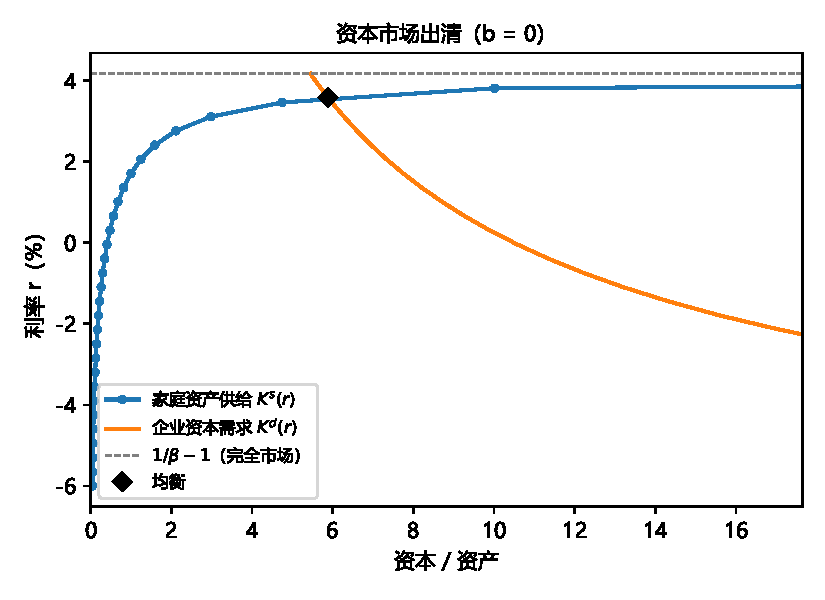
\includegraphics[width=\textwidth]{aiyagari_borrowing_capital_market.pdf}
\caption{资本市场出清（$b=0$）。蓝线为家庭净资产供给 $K^s(r)$，橙线为企业资本需求 $K^d(r)$，虚线为完全市场利率 $1/\beta-1$，菱形为均衡点。横轴为资本（资产），纵轴为年利率（\%）}\label{fig:cm}
\end{minipage}\hfill
\begin{minipage}{0.48\textwidth}\centering
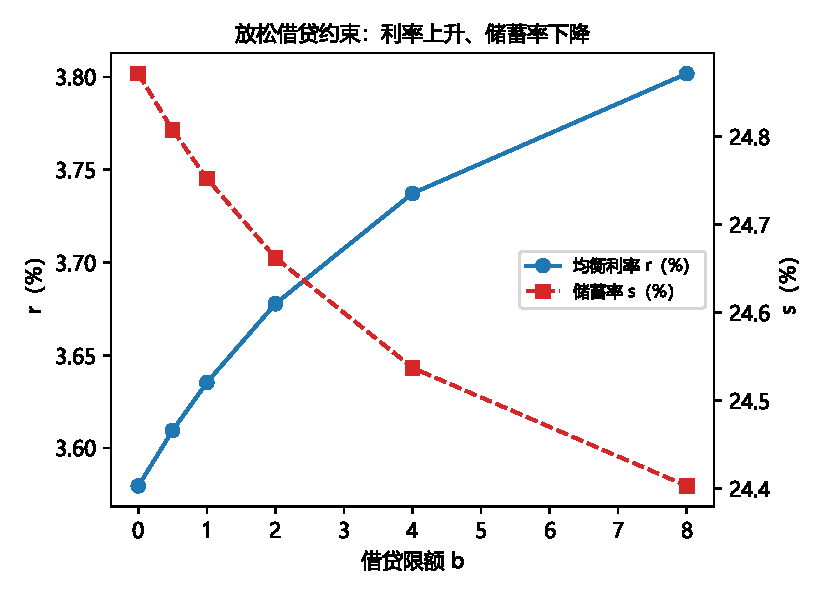
\includegraphics[width=\textwidth]{aiyagari_borrowing_comparative_statics.pdf}
\caption{借贷限额的比较静态。横轴为借贷限额 $b$；蓝线（左轴）为均衡年利率（\%），红线（右轴）为储蓄率 $s=\delta K/Y$（\%）}\label{fig:cs}
\end{minipage}
\end{figure}

\begin{figure}[h]
\centering
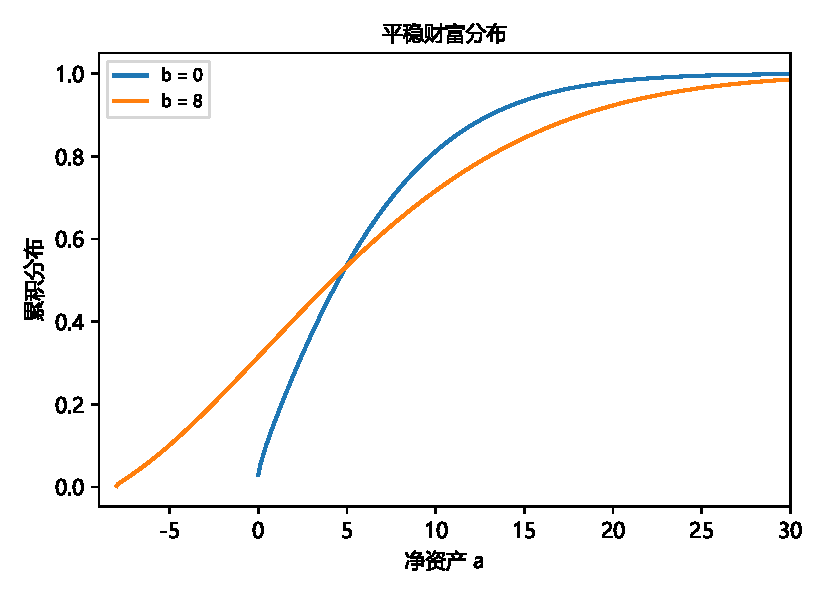
\includegraphics[width=0.55\textwidth]{aiyagari_borrowing_wealth_distribution.pdf}
\caption{平稳财富分布的累积分布函数（$b=0$ 与 $b=8$）。横轴为净资产 $a$，纵轴为累积人口比例；$b=8$ 时分布下端延伸至负值区域}\label{fig:wd}
\end{figure}

\section{稳健性}

表~\ref{tab:rob} 比较不同的收入离散化方法与状态数。Rouwenhorst 方法下，状态数从 7 增加到 15，利率变化不超过 0.002 个百分点、储蓄率变化不超过 0.004 个百分点，说明结果对状态数不敏感。Tauchen 方法（7 状态、网格宽度 3 个标准差，Tauchen 1986）把对数收入方差高估约 37\%，使预防性储蓄被高估：零借贷下利率为 3.371\%，比 Rouwenhorst 结果低约 0.21 个百分点。两种方法下比较静态的方向相同，但 Tauchen 方法夸大了幅度。

\begin{table}[h]
\centering\small
\caption{收入过程离散化的稳健性。方差相对误差为离散后对数收入的无条件方差相对目标值 $\sigma^2=0.04$ 的偏差}\label{tab:rob}
\begin{tabular}{lrrrrr}
\toprule
离散化方法 & 状态数 & $b$ & $r$（\%） & $s$（\%） & 对数收入方差相对误差（\%） \\
\midrule
Rouwenhorst & 7 & 0 & 3.580 & 24.87 & 0.0 \\
Rouwenhorst & 15 & 0 & 3.578 & 24.87 & 0.0 \\
Tauchen & 7 & 0 & 3.371 & 25.33 & 37.1 \\
\midrule
Rouwenhorst & 7 & 2 & 3.678 & 24.66 & 0.0 \\
Rouwenhorst & 15 & 2 & 3.676 & 24.67 & 0.0 \\
\midrule
Rouwenhorst & 7 & 8 & 3.802 & 24.40 & 0.0 \\
Rouwenhorst & 15 & 8 & 3.800 & 24.41 & 0.0 \\
Tauchen & 7 & 8 & 3.668 & 24.68 & 37.1 \\
\bottomrule
\end{tabular}

\end{table}

\section{总结与局限}

在 Aiyagari 经济中，不可保险的收入风险使均衡利率低于、储蓄率高于完全市场水平；在所考察的范围内，放宽借贷约束使利率上升、资本产出比与储蓄率下降、受约束家庭比例下降。这些结论在 Rouwenhorst 离散下对状态数不敏感，但离散化方法会影响水平与幅度，高持续性收入过程应避免使用粗糙的 Tauchen 离散。

本文的比较静态只比较稳态，未计算过渡路径与福利；劳动供给无弹性，无政府与总量冲击；未与 Aiyagari (1994) 原文表格逐格对照，而以收入风险趋于零的极限情形作为可验证的基准。

\begin{thebibliography}{9}
\bibitem{a94} Aiyagari, S. R. (1994). Uninsured idiosyncratic risk and aggregate saving. \textit{Quarterly Journal of Economics}, 109(3), 659--684.
\bibitem{c06} Carroll, C. D. (2006). The method of endogenous gridpoints for solving dynamic stochastic optimization problems. \textit{Economics Letters}, 91(3), 312--320.
\bibitem{h93} Huggett, M. (1993). The risk-free rate in heterogeneous-agent incomplete-insurance economies. \textit{Journal of Economic Dynamics and Control}, 17(5--6), 953--969.
\bibitem{k10} Kopecky, K. A., \& Suen, R. M. H. (2010). Finite state Markov-chain approximations to highly persistent processes. \textit{Review of Economic Dynamics}, 13(3), 701--714.
\bibitem{t86} Tauchen, G. (1986). Finite state Markov-chain approximations to univariate and vector autoregressions. \textit{Economics Letters}, 20(2), 177--181.
\bibitem{y10} Young, E. R. (2010). Solving the incomplete markets model with aggregate uncertainty using the Krusell--Smith algorithm and non-stochastic simulations. \textit{Journal of Economic Dynamics and Control}, 34(1), 36--41.
\end{thebibliography}

\end{document}
